\chapter{Dissection}{B}
\label{app:dissection}
Dissection of the crab is done in two parts; first the gross dissection and then the fine dissection. During the gross dissection the entire stomach is removed from the crab, and during the fine dissection the \ac{STNS} is extracted from the stomach and pinned in a Petri dish. During both parts of the dissection the preparation is kept cool by replacing the saline every 10 minutes with fresh saline from the fridge. A basic anatomy of the  whole crab and the stomach is shown in figure \ref{fig:dissectionimage} and \ref{fig:stomach}.

\begin{figure}[H]
	\begin{center}
		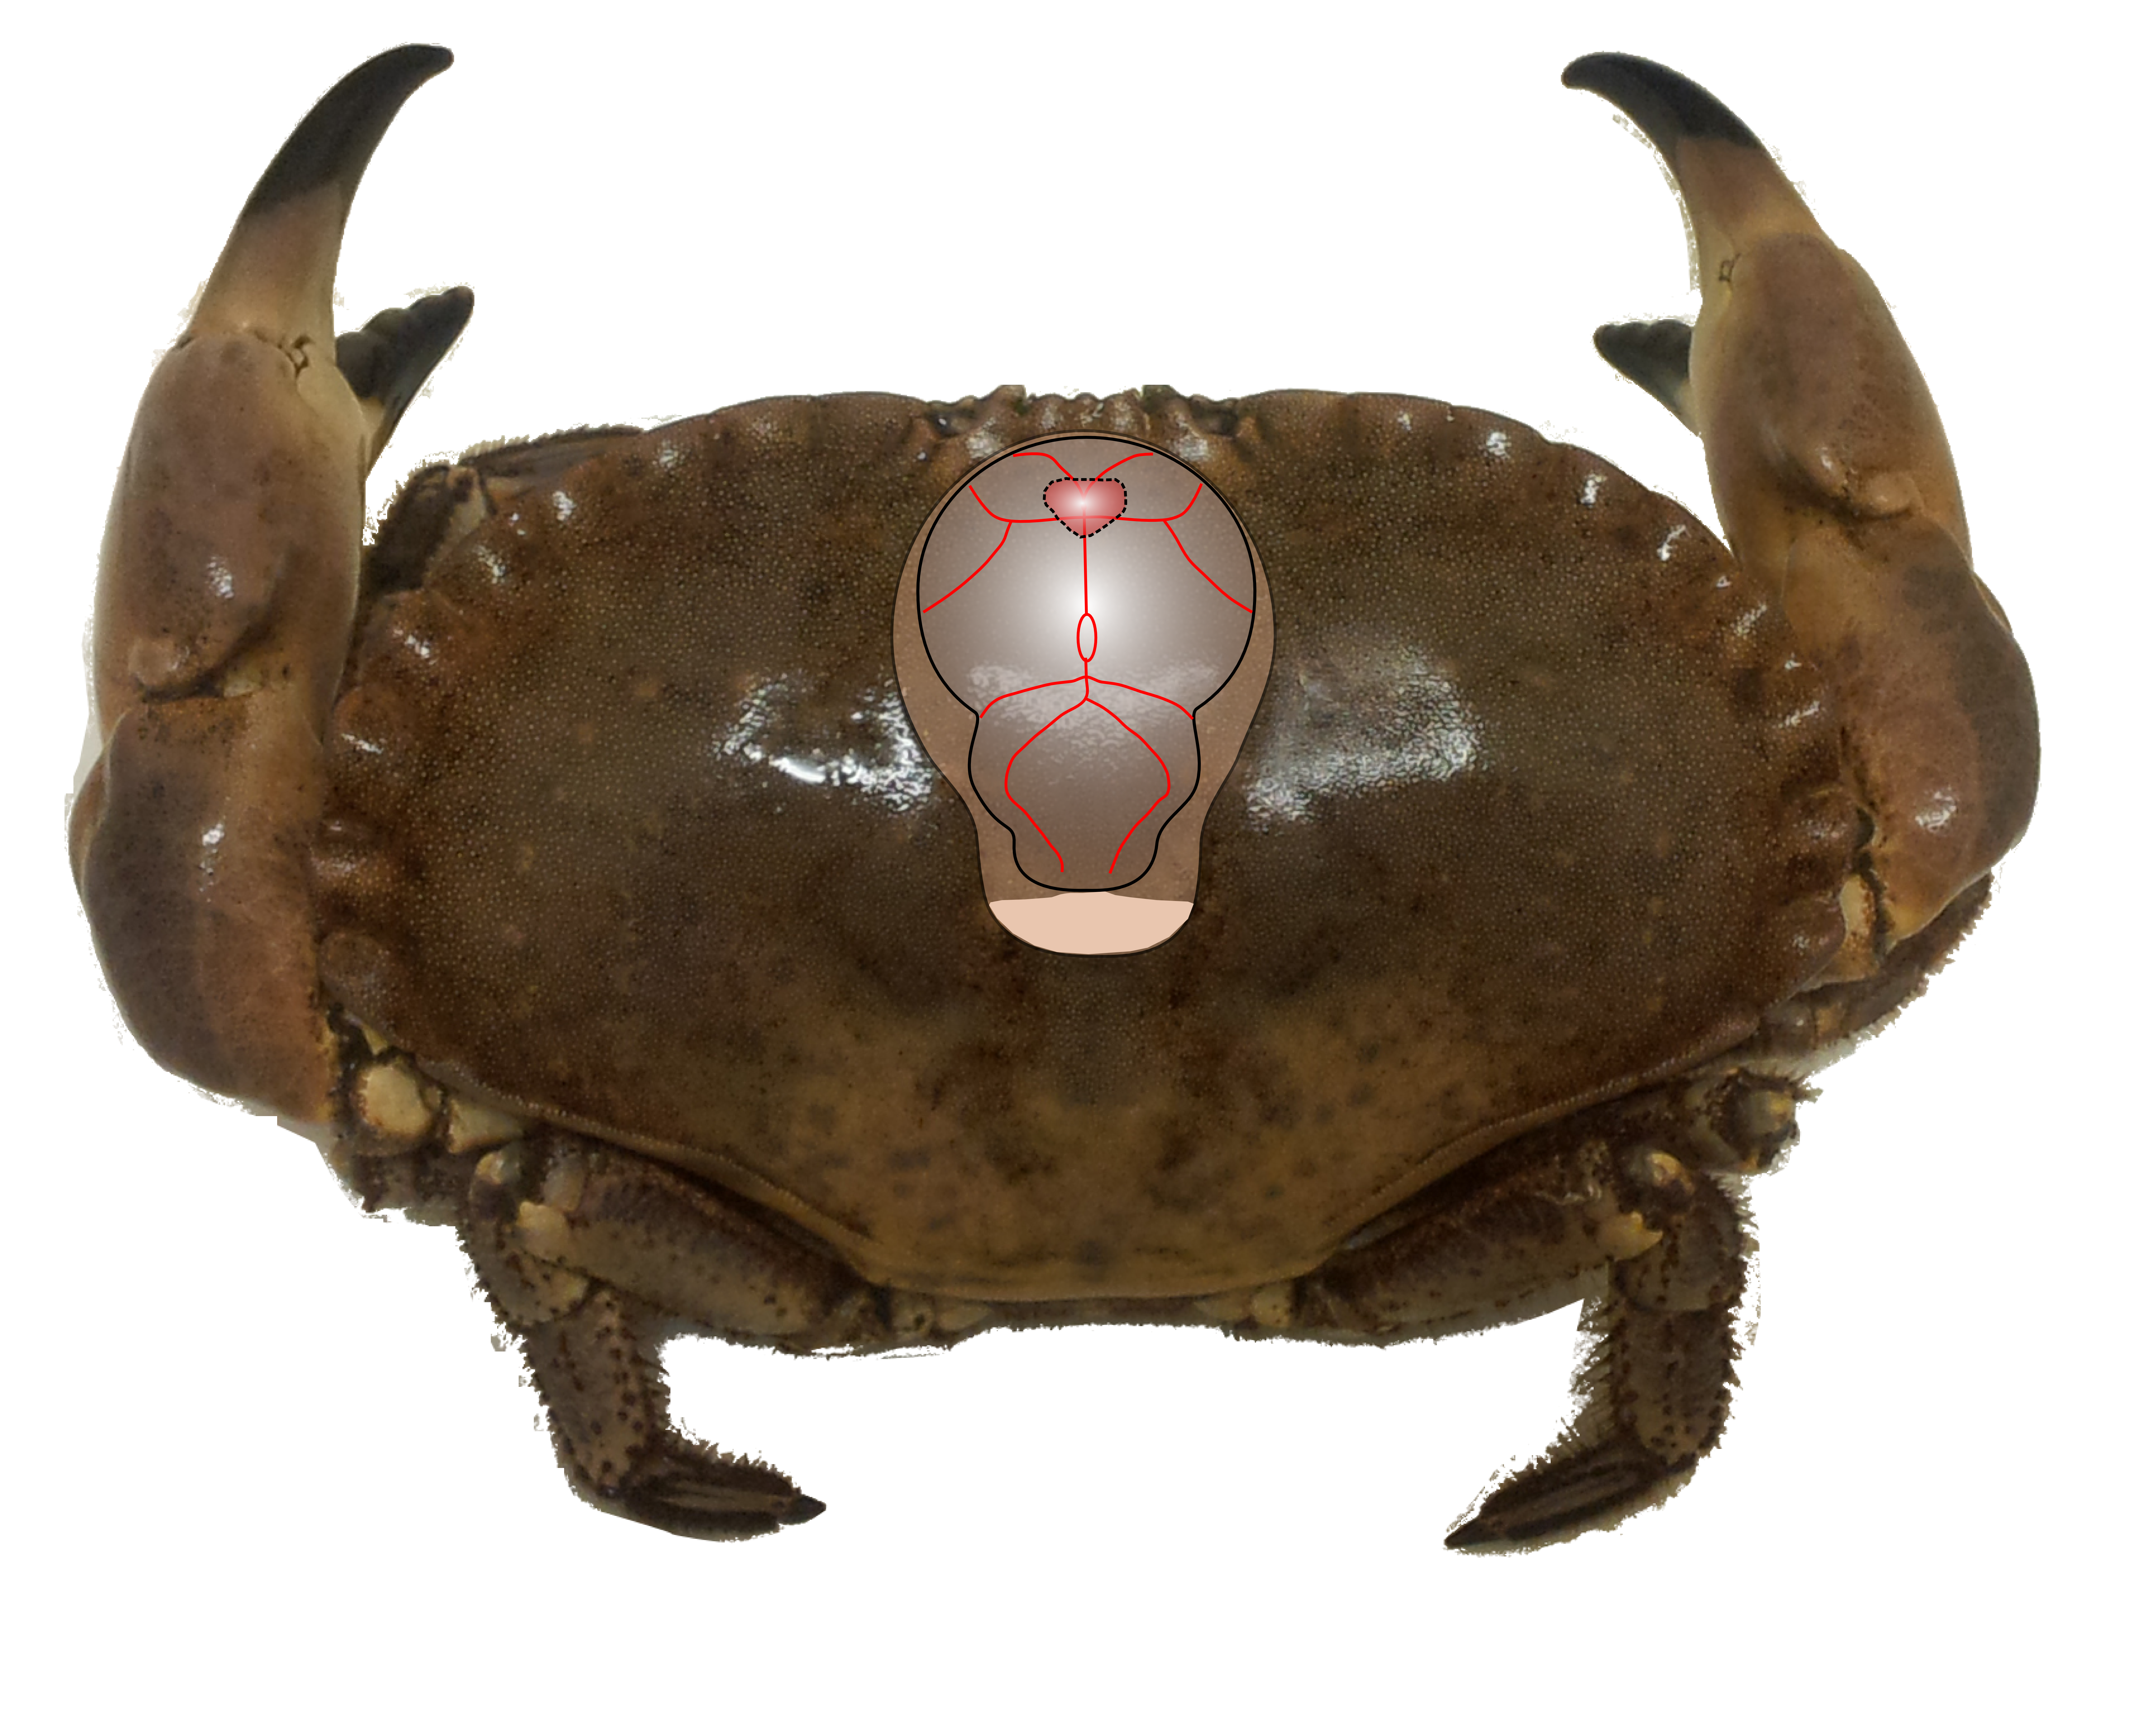
\includegraphics[width=8cm]{graphics/dissectionimage.png}
		\caption{The basic anatomy of the crab showing the location of the stomach. (Adapted from \cite{Stein2009})}
		\label{fig:dissectionimage}
	\end{center}
\end{figure}

\begin{figure}[H]
	\begin{center}
		\includegraphics[width=9cm]{graphics/stomach.png}
		\caption{The stomach of the crab with the \ac{STNS}. (Adapted from \cite{Stein2009})}
		\label{fig:stomach}
	\end{center}
\end{figure}



\section{Gross dissection}
The dissection process is started by anaesthetising a crab on ice for about 30 to 45 minutes. A dissection pan is laid out with the tools required, which are; rongeurs, a tapered edge spatula, small scissors, toothed forceps and a black Sylgard-coated dish. Insect pins are used to pin the preparation down. Crab saline (Table \ref{tab:saline}) is also required. Gloves are worn when handling the crabs.

% Table generated by Excel2LaTeX from sheet 'Sheet1'
\begin{table}[H]
	\centering
	\caption{\species{Cancer pagurus} saline}
	\label{tab:saline}
	\begin{tabular}{lrrrrr}
		\hline 
		\textbf{Salt} & \textbf{(mM)} & \textbf{g/Liter} & \textbf{g/2 Liter} & \textbf{g/5 Liter} & \textbf{g/8 Liter} \\ \hline
		KCl   & 11.00    & 0.83  & 1.66  & 4.15  & 6.64 \\
		NaCl  & 440.00   & 25.80  & 51.60  & 129.00   & 206.40 \\
		CaCl2H2O & 13.00    & 1.90   & 3.80   & 9.50   & 15.20 \\
		MgCl26H2O & 26.00    & 5.30   & 10.60  & 26.50  & 42.40 \\
		Trizma base & 11.2  &  1.50  &  3.00  &  7.30  &  12.00 \\
		Maleic Acid &  5.00  &  0.60  &  1.20  &  3.00  &  4.80 \\
		Hepes &  10.00 &  2.38 &  4.76 &  9.52 & 19.04 \\
		\multicolumn{6}{l}{\textit{(Hepes can be used instead of Tris+Maleate)}} \\
		\hline
	\end{tabular}%
\end{table}%

The first step is to remove the claws and legs using rongeurs or manually (Fig. \ref{fig:dissection_crab2}).

\begin{figure}[H]
	\begin{center}
		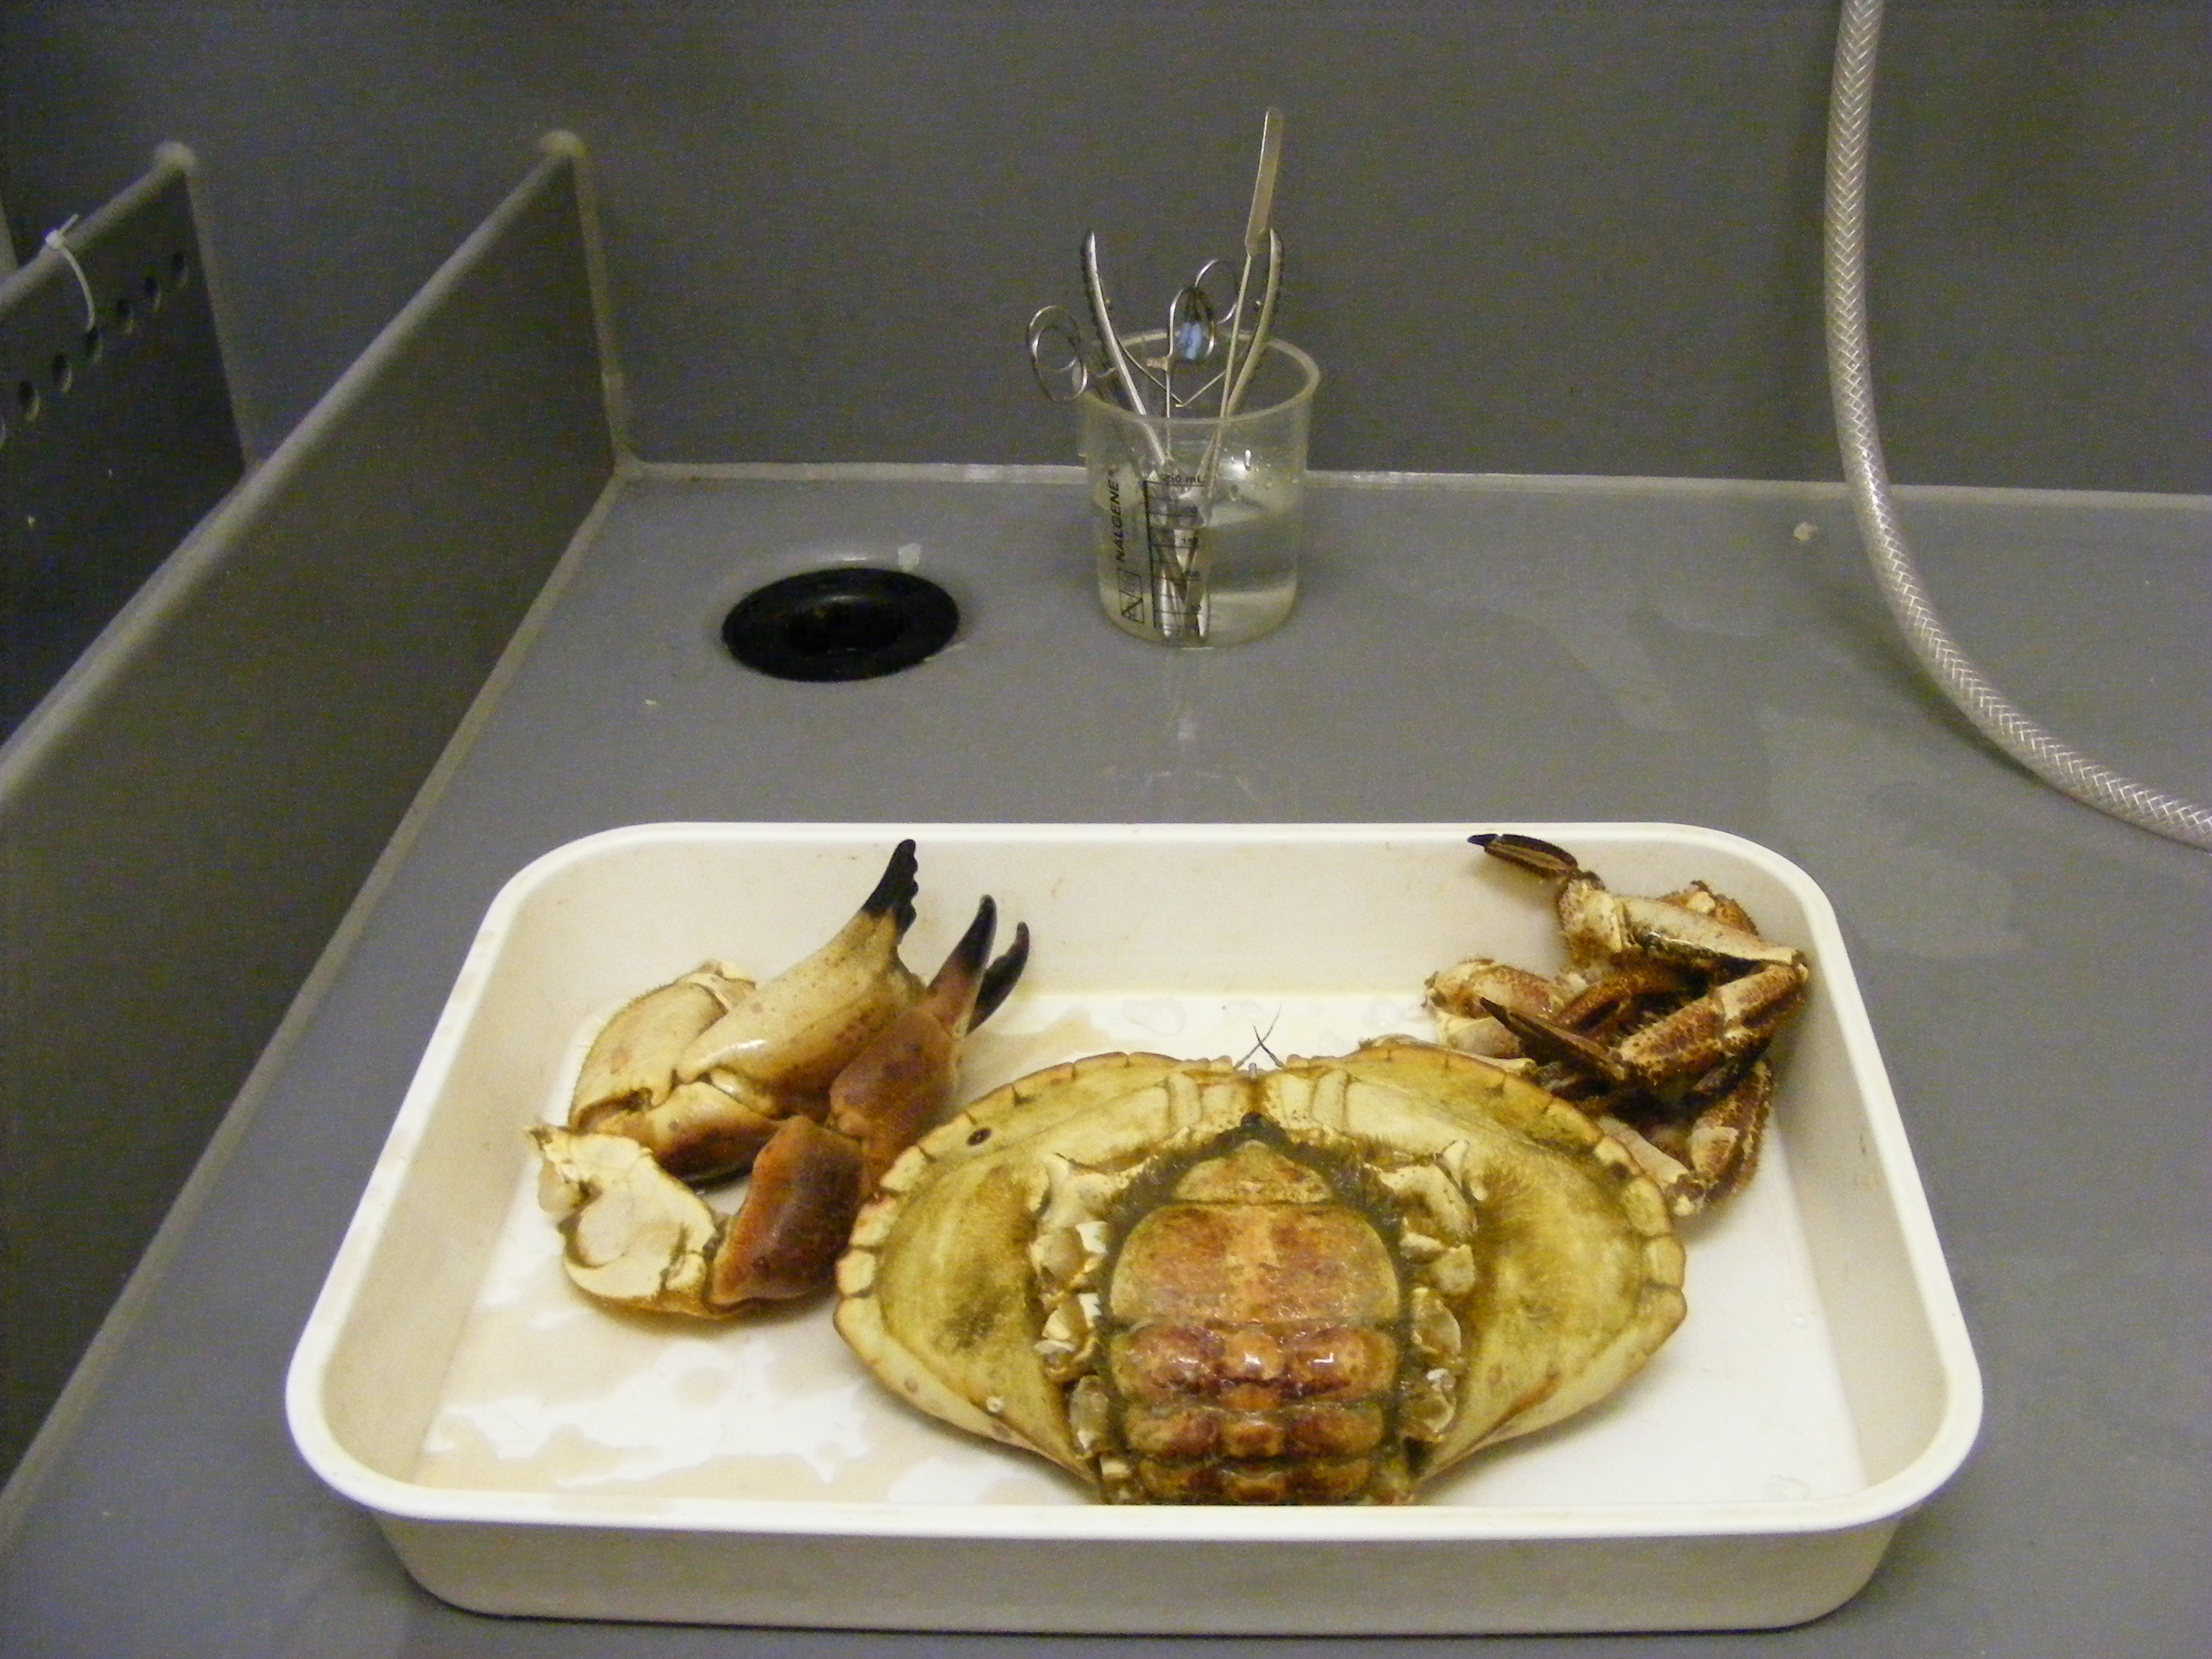
\includegraphics[width=9cm]{graphics/dissection_crab2.png}
		\caption{First step of dissections is to remove the claws and legs using rongeurs or manually.}
		\label{fig:dissection_crab2}
	\end{center}
\end{figure}

The external mouth parts are removed next. Using the rongeurs the large external mandibles are removed first and then the smaller 1st and 2nd maxillipeds, exposing the 2nd maxillae which covers the opening to the oesophagus. The 2nd maxillae are attached to thin long ossicles with a muscle attached to the end. These are removed, using the rongeurs, with a twist and pull motion.

The rongeurs are then used to break off the carapace edges on both sides by starting at the lateral posterior end and working towards, and up to the eyes. A gap is created between the dorsal and ventral carapace, exposing the hypodermis (Fig. \ref{fig:dissection_crab3}).

\begin{figure}[H]
	\begin{center}
		\includegraphics[width=9cm]{graphics/dissection_crab3.png}
		\caption{Removing the frilled edge on the side of the carapace, exposing the hypodermis underneath.}
		\label{fig:dissection_crab3}
	\end{center}
\end{figure}

Eyes, antennae and rostrum are chipped away leaving a thin layer of carapace intact that can later be easily broken by hand. 

The hypodermis is then separated from the carapace, holding the spatula against carapace so as to not put pressure on the tissue below in which the \ac{STNS} is embedded (Fig. \ref{fig:dissection_crab4}).

\begin{figure}[H]
	\begin{center}
		\includegraphics[width=9cm]{graphics/dissection_crab4.png}
		\caption{The hypodermis is separated from the carapace taking care not to damage the tissue below the carapace where the nervous system is located.}
		\label{fig:dissection_crab4}
	\end{center}
\end{figure}

The carapace is removed in three sections (Fig. \ref{fig:dissection_crab_sections}). The triangular shapes on the sides are removed first (Fig. \ref{fig:dissection_crab5}). The tapered edge of the spatula is then used again to separate the hypodermis from the centre part that is left over when side sections have been removed. %(Fig \ref{fig:dissection_crab6}). 
The hypodermis is separated from the carapace as far forward (anteriorly) as possible and as far back (posteriorly) as the two ossicles that protrude from the carapace. The centre part of the carapace is then be removed by breaking the connecting strip  of carapace parallel to the posterior and between the two  corners of the triangular shaped sections. This section is then removed manually by bending it upwards towards the anterior, exposing almost all of the hypodermis on the dorsal side of the crab (Fig. \ref{fig:dissection_crab7}).

\begin{figure}[H]
	\begin{center}
		\includegraphics[width=9cm]{graphics/dissection_crab_sections.png}
		\caption{The carapace is removed in three sections.}
		\label{fig:dissection_crab_sections}
	\end{center}
\end{figure}
\begin{figure}[H]
	\begin{center}
		\includegraphics[width=9cm]{graphics/dissection_crab5.png}
		\caption{Firstly the triangular shaped section to the sides are removed.}
		\label{fig:dissection_crab5}
	\end{center}
\end{figure}

\begin{figure}[H]
	\begin{center}
		\includegraphics[width=9cm]{graphics/dissection_crab6.png}
		\caption{The centre part of the carapace should be separated from the hypodermis until one can see through the opening.}
		\label{fig:dissection_crab6}
	\end{center}
\end{figure}
\begin{figure}[H]
	\begin{center}
		\includegraphics[width=9cm]{graphics/dissection_crab7.png}
		\caption{The last section of carapace to be removed is the centre part.}
		\label{fig:dissection_crab7}
	\end{center}
\end{figure}

The tapered edge of the spatula is then used to separate ventral tissue from the carapace. Tissue at the cephalon is drawn back exposing the connecting tissue (Fig. \ref{fig:dissection_crab8}). The connecting tissue is then cut with the scissors allowing the tissue to be drawn back even further - up to the point where the oesophagus is attached to the ventral side of the carapace is exposed (Fig. \ref{fig:dissection_crab9}).

\begin{figure}[H]
	\begin{center}
		\includegraphics[width=9cm]{graphics/dissection_crab8.png}
		\caption{Separate the ventral tissue from the carapace and push the tissue below the eyes as far back as the connecting tissue.}
		\label{fig:dissection_crab8}
	\end{center}
\end{figure}
\begin{figure}[H]
	\begin{center}
		\includegraphics[width=9cm]{graphics/dissection_crab9.png}
		\caption{The connecting tissue is cut using the scissors and push the tissue back up to where the top oesophagus is exposed.}
		\label{fig:dissection_crab9}
	\end{center}
\end{figure}

The labrum is detached from the epistome using small scissors. The cephalum is then removed making diagonal breaks from next to the eyes down to the oesophagus (Fig. \ref{fig:dissection_crab10})

\begin{figure}[H]
	\begin{center}
		\includegraphics[width=9cm]{graphics/dissection_crab10.png}
		\caption{The cephalum is removed after the oesophagus is loosened from the carapace and then diagonal breaks are made from the eyes to the oesophagus.}
		\label{fig:dissection_crab10}
	\end{center}
\end{figure}

The crab is then propped up on the side of the dissection pan using the claws. While the labrum is held in place with the forceps the stomach is extracted by cutting it away from the ventral carapace (Fig. \ref{fig:dissection_crab11}).

\begin{figure}[H]
	\begin{center}
		\includegraphics[width=9cm]{graphics/dissection_crab11.png}
		\caption{The crab is propped up on the side of the dissection pan using the claws. While the labrum is held in place with the forceps the stomach is extracted by cutting it away from the ventral carapace.}
		\label{fig:dissection_crab11}
	\end{center}
\end{figure}

The stomach is then removed from the body and laid down the back of the hand with the hypodermis facing down (Fig. \ref{fig:dissection_crab12}). 
\begin{figure}[H]
	\begin{center}
		\includegraphics[width=9cm]{graphics/dissection_crab12.png}
		\caption{The stomach is removed from the body and laid down the back of the hand with the hypodermis facing down.}
		\label{fig:dissection_crab12}
	\end{center}
\end{figure}
Excess tissue is scraped off and then the stomach is filled with saline to inflate it. Inflating the stomach with saline makes it easier to enter the scissors into the oesophagus to cut through the top layer of the stomach from the oesophagus to the pylorus and through the ossicle between the ampullae (Fig. \ref{fig:dissection_crab13}). 
\begin{figure}[H]
	\begin{center}
		\includegraphics[width=9cm]{graphics/dissection_crab13.png}
		\caption{A cut is made from the oesophagus to the pylorus.}
		\label{fig:dissection_crab13}
	\end{center}
\end{figure}
Two diagonal cuts are made through the cardial branches, which allows the stomach to open up and expose the three teeth inside. The tips of three teeth are cut off (Fig. \ref{fig:dissection_crab14}) which allows the stomach to lie flat when placed in a dish with black Sylgard and the inside of the stomach facing down. The dish is filled with cold crab saline before the stomach is placed in it. The stomach lining is pinned down tightly using dissection pins (Fig. \ref{fig:dissection_crab15}).
\begin{figure}[H]
	\begin{center}
		\includegraphics[width=9cm]{graphics/dissection_crab14.png}
		\caption{The tips of the three teeth are cut off.}
		\label{fig:dissection_crab14}
	\end{center}
\end{figure}
\begin{figure}[H]
	\begin{center}
		\includegraphics[width=9cm]{graphics/dissection_crab15.png}
		\caption[Pinned-down stomach. ]{\textbf{Pinned-down stomach. }The opened stomach is pinned down flat in a dish with black Sylgard. The inside of the stomach faces down. Before the stomach is placed in the dish the dish is filled with crab saline. }
		\label{fig:dissection_crab15}
	\end{center}
\end{figure}

\section{Fine dissection}

For the fine dissection the following additional equipment is needed, a stereoscopic microscope with zoom capability, a 3.5 inch clear Sylgard coated petri dish, two size 5 forceps, dissecting scissors, small dissection pins, fine dissection pins and saline.

When viewed from above the dissected stomach is covered with hypodermis. More or less in the middle of the preparation there are two small dots. All of the hypodermis is cut away leaving only a small circle of tissue around the two dots.

% (Fig. \ref{fig:finedissection_crab01})
%\begin{figure}[H]
%	\begin{center}
%		\includegraphics[width=9cm]{graphics/figure_x.png}
%		\caption{Cut all of the hypodermis away leaving only a small circle around the two dots in the middle of the prep.}
%		\label{fig:finedissection_crab01}
%	\end{center}
%\end{figure}
To the anterior of the small piece of hypodermic tissue left behind, is the brain. From the brain there are two thick nerves, the \ac{coc} nerves. Covering these nerves is a layer of light yellow tissue, which when cut away, makes it possible to see the \ac{coc} well enough through the. Starting at the brain the \acp{coc} are exposed by following them and cutting the tissue above to expose the nerve. The nerve is followed to expose the \acp{CoG} and the rest of the nerve to the anterior of the preparation where the nerve ends. All tissue to the posterior of the \acp{coc} is cleared away. The brain is then lifted and the tissue below the brain and above the opthalmic artery is cut away. The \acp{coc} are then cut against the brain and the brain is removed. Once the brain is removed it is possible to see the opthalmic artery clearly. The opthalmic artery splits to form a 'Y'. By grasping the artery with the forceps to the posterior of the split it is possible to lift the artery and see where the \ac{stn} leaves the artery and bends downward. The artery is cut as close to the \ac{stn} as possible and is then removed by cutting it away from the tissue below and cutting it loose from the ossicles to the the anterior. With the artery removed it is possible to the see the \ac{OG} and the \acp{ion}. To clear the \acp{ion} they are followed from both the \ac{OG} and \acp{CoG}. As one follows the \acp{ion} to be cleared, care has to be taken to notice the where the labral nerve splits off. All tissue between the \acp{ion} is cleared away ass well as the tissue to the anterior of the ions.

At this point in the dissection it is also possible to see the \acp{son} splitting of the \ac{stn}. The \acp{son} can be followed and exposed from the \ac{stn} towards the \acp{CoG}. The tissue between the \acp{son} and \acp{ion} can be clear away leaving only the exposed nerves behind. The \acp{dpon} split off the \ac{son} and care has to be taken to leave at least a short stub of the \ac{dpon} behind for pinning the preparation down in the petri dish later on.

It is now also possible to clear away all orange coloured glandular tissue to the sides of the ac{stn}, posteriorly of the \acp{son}. The are below the \ac{stn} is covered by white tissue that resembles white "wadding" (the material used to stuff padded clothing). The \acp{mvn} run below the orange glandular tissue and on the edge of the white tissue. About two to three centimetres of the \acp{mvn} are cleared. It can sometime be quite difficult to see the white nerves running inside this white tissue but by zooming in on the nerves it is possible to follow the \ac{dvn} (the nerve projecting posteriorly from the \ac{STG}). The \ac{dgn} usually projects out of the \ac{STG} or splits off the \ac{dvn} and then bends downwards towards the dorsal side of the preparation. One to two centimetres of the \ac{dgn} is left in tact and cleared. The \ac{dvn} splits into two ac{lvn}, both which have to be exposed by following them to the posterior and, if possible, to where they split into the \ac{pyn} and \ac{pdn}

Once all these nerves are exposed, care is taken to cut the nervous system away from any tissue that might still be attaching it to the tissue ventrally of the \ac{STNS}. If not already detached, the ends of the \acp{coc}, labral nerves, \acp{dpon}, \acp{mvn}, \ac{dgn} and \ac{lvn},\acp{pyn}, \acp{pdn} are cut loose. The whole \ac{STNS} can now be lifted by grasping it by the ends of the \ac{coc} and the \acp{lvn} and moving it to the side of the dish. The left over stomach lining is unpinned and used to rub it over the Sylgard lined petri dish. Sylgard is hydrophobic and the water will form puddles and not spread evenly over the Sylgard if it is not conditioned in this way with the stomach. Also, without the conditioning the nerves will strongly adhere to the Sylgard and become impossible to handle without damaging. The Petri dish is then rinsed in filled with saline. Grasping the nerves as before, the nervous system is then transferred into the Petri dish. The \ac{STNS} is pinned down onto the Sylgard using minuten pins.

The \ac{STG} can now be exposed by grasping the hypodermis that was left behind with the forceps and lifting it up. This exposes an opening into the ophthalmic artery. The artery is split open by entering the scissors into the artery opening and cutting from the posterior to the anterior between the two dots on the hypodermis. The cut has to be made all the way to the anterior where the artery was cut earlier. Because the artery tissue can be quite tough the artery is sometimes pinned down to the sides to create enough tension for the scissors to cut. The cuts are made while slightly pulling upwards to avoid touching or damaging the STG and the \ac{stn} which runs along the bottom of the artery. Once the \ac{stn} and ac{STG} are exposed the excess artery and hypodermic tissue can be cut away to only leave behind the exposed nerves. Care is taken when the tissue is cut away to leave small stubs of \acp{aln} behind which are required to pin down the \ac{STG}. Without the \acp{aln} it is very difficult to pin the \ac{STG} down sufficiently when desheathing the \ac{STG}.

All excess tissue is cleared away from the \ac{STNS}.



